% Options for packages loaded elsewhere
% Options for packages loaded elsewhere
\PassOptionsToPackage{unicode}{hyperref}
\PassOptionsToPackage{hyphens}{url}
%
\documentclass[
  ignorenonframetext,
  aspectratio=169,
  russian,
]{beamer}
\newif\ifbibliography
\usepackage{pgfpages}
\setbeamertemplate{caption}[numbered]
\setbeamertemplate{caption label separator}{: }
\setbeamercolor{caption name}{fg=normal text.fg}
\beamertemplatenavigationsymbolshorizontal
% remove section numbering
\setbeamertemplate{part page}{
  \centering
  \begin{beamercolorbox}[sep=16pt,center]{part title}
    \usebeamerfont{part title}\insertpart\par
  \end{beamercolorbox}
}
\setbeamertemplate{section page}{
  \centering
  \begin{beamercolorbox}[sep=12pt,center]{section title}
    \usebeamerfont{section title}\insertsection\par
  \end{beamercolorbox}
}
\setbeamertemplate{subsection page}{
  \centering
  \begin{beamercolorbox}[sep=8pt,center]{subsection title}
    \usebeamerfont{subsection title}\insertsubsection\par
  \end{beamercolorbox}
}
% Prevent slide breaks in the middle of a paragraph
\widowpenalties 1 10000
\raggedbottom
\AtBeginPart{
  \frame{\partpage}
}
\AtBeginSection{
  \ifbibliography
  \else
    \frame{\sectionpage}
  \fi
}
\AtBeginSubsection{
  \frame{\subsectionpage}
}
\usepackage{iftex}
\ifPDFTeX
  \usepackage[T1]{fontenc}
  \usepackage[utf8]{inputenc}
  \usepackage{textcomp} % provide euro and other symbols
\else % if luatex or xetex
  \usepackage{unicode-math} % this also loads fontspec
  \defaultfontfeatures{Scale=MatchLowercase}
  \defaultfontfeatures[\rmfamily]{Ligatures=TeX,Scale=1}
\fi
\usepackage{lmodern}

\usetheme[]{metropolis}
\usefonttheme{serif} % use mainfont rather than sansfont for slide text
\ifPDFTeX\else
  % xetex/luatex font selection
  \setmainfont[]{DejaVu Sans}
  \setsansfont[]{DejaVu Sans}
  \setmonofont[]{DejaVu Sans Mono}
\fi
% Use upquote if available, for straight quotes in verbatim environments
\IfFileExists{upquote.sty}{\usepackage{upquote}}{}
\IfFileExists{microtype.sty}{% use microtype if available
  \usepackage[]{microtype}
  \UseMicrotypeSet[protrusion]{basicmath} % disable protrusion for tt fonts
}{}


\usepackage{longtable,booktabs,array}
\newcounter{none} % for unnumbered tables
\usepackage{calc} % for calculating minipage widths
\usepackage{caption}
% Make caption package work with longtable
\makeatletter
\def\fnum@table{\tablename~\thetable}
\makeatother
\usepackage{graphicx}
\makeatletter
\newsavebox\pandoc@box
\newcommand*\pandocbounded[1]{% scales image to fit in text height/width
  \sbox\pandoc@box{#1}%
  \Gscale@div\@tempa{\textheight}{\dimexpr\ht\pandoc@box+\dp\pandoc@box\relax}%
  \Gscale@div\@tempb{\linewidth}{\wd\pandoc@box}%
  \ifdim\@tempb\p@<\@tempa\p@\let\@tempa\@tempb\fi% select the smaller of both
  \ifdim\@tempa\p@<\p@\scalebox{\@tempa}{\usebox\pandoc@box}%
  \else\usebox{\pandoc@box}%
  \fi%
}
% Set default figure placement to htbp
\def\fps@figure{htbp}
\makeatother



\ifLuaTeX
\usepackage[bidi=basic,shorthands=off,provide=*]{babel}
\else
\usepackage[bidi=default,shorthands=off,provide=*]{babel}
\fi
\ifPDFTeX
\else
\babelfont{rm}[]{DejaVu Sans}
\fi
\ifLuaTeX
  \usepackage{selnolig} % disable illegal ligatures
\fi


\setlength{\emergencystretch}{3em} % prevent overfull lines

\providecommand{\tightlist}{%
  \setlength{\itemsep}{0pt}\setlength{\parskip}{0pt}}



 

\usepackage[]{csquotes}

%%% Load theme
\IfFileExists{beamerthemegotham.sty}{
  %%%% Full TeXlive
  \usetheme{gotham}
  \gothamset{
    numbering=totalframenumber,
    parttocframe default=off,
    sectiontocframe default=off,
    subsectiontocframe default=off,
    tocframe template=gotham bullet,
    % progressbar position=frametitle,
    progressbar position=foot,
  }
  \renewcommand{\gothamInstituteLogoSquare}[1][4ex]{%
    
\includegraphics[height=##1]{_resources/image/logo_rudn-inverted.png}
  }
  % \renewcommand{\gothamtitlepagelogo}[1][4ex]{%
  %   
\includegraphics[height=##1]{_resources/image/logo_rudn.png}
  % }
}{%
  %%%% TinyTeX
  \usepackage{libertine}
  %%%% https://deic.uab.cat/~iblanes/beamer_gallery/
  \usetheme{Madrid}
}
\metroset{progressbar=frametitle,numbering=fraction}
\makeatletter
\@ifpackageloaded{caption}{}{\usepackage{caption}}
\AtBeginDocument{%
\ifdefined\contentsname
  \renewcommand*\contentsname{Содержание}
\else
  \newcommand\contentsname{Содержание}
\fi
\ifdefined\listfigurename
  \renewcommand*\listfigurename{Список иллюстраций}
\else
  \newcommand\listfigurename{Список иллюстраций}
\fi
\ifdefined\listtablename
  \renewcommand*\listtablename{Список таблиц}
\else
  \newcommand\listtablename{Список таблиц}
\fi
\ifdefined\figurename
  \renewcommand*\figurename{Рисунок}
\else
  \newcommand\figurename{Рисунок}
\fi
\ifdefined\tablename
  \renewcommand*\tablename{Таблица}
\else
  \newcommand\tablename{Таблица}
\fi
}
\@ifpackageloaded{float}{}{\usepackage{float}}
\floatstyle{ruled}
\@ifundefined{c@chapter}{\newfloat{codelisting}{h}{lop}}{\newfloat{codelisting}{h}{lop}[chapter]}
\floatname{codelisting}{Список}
\newcommand*\listoflistings{\listof{codelisting}{Листинги}}
\makeatother
\makeatletter
\makeatother
\makeatletter
\@ifpackageloaded{caption}{}{\usepackage{caption}}
\@ifpackageloaded{subcaption}{}{\usepackage{subcaption}}
\makeatother

\usepackage{bookmark}
\IfFileExists{xurl.sty}{\usepackage{xurl}}{} % add URL line breaks if available
\urlstyle{same}
% fallback for those not using the hyperref driver hyperxmp:
\makeatletter
\@ifundefined{xmpquote}{\newcommand{\xmpquote}[1]{#1}}{}
\makeatother
\hypersetup{
  pdftitle={Лабораторная работа №2},
  pdfauthor={Нечаева Кира Андреевна},
  pdflang={ru-RU},
  hidelinks,
  pdfcreator={LaTeX via pandoc}}


\title{\texorpdfstring{Лабораторная работа №2}{Лабораторная работа №2}}
\subtitle{\texorpdfstring{Задача о погоне}{Задача о погоне}}
\author{Нечаева Кира Андреевна}
\date{Invalid Date}
\institute{НКНбд-01-23}

\begin{document}
\frame{\titlepage}


\begin{frame}{Постановка задачи}
\protect\phantomsection\label{ux43fux43eux441ux442ux430ux43dux43eux432ux43aux430-ux437ux430ux434ux430ux447ux438}
\textbf{Вариант 2}

Начальное расстояние:

\[
k=12\text{ км}.
\]

Скорость катера в \textbf{4 раза больше} скорости лодки.

Необходимо:

\begin{itemize}
\tightlist
\item
  получить уравнение движения катера;
\item
  рассмотреть два начальных положения;
\item
  построить траектории;
\item
  определить точки встречи.
\end{itemize}
\end{frame}

\begin{frame}{Математическая модель}
\protect\phantomsection\label{ux43cux430ux442ux435ux43cux430ux442ux438ux447ux435ux441ux43aux430ux44f-ux43cux43eux434ux435ux43bux44c}
Для первого случая:

\[
r_0=\frac{12}{4+1}=2.4\text{ км}.
\]

Для второго:

\[
r_0=\frac{12}{4-1}=4\text{ км}.
\]

Уравнение дальнейшего движения:

\[
\boxed{
\frac{dr}{d\theta}=\frac{r}{\sqrt{15}}
}
\]

Начальные условия:

\[
(\theta_0,r_0)=(0,2.4)
\]

\[
(\theta_0,r_0)=(-\pi,4)
\]
\end{frame}

\begin{frame}{Реализация}
\protect\phantomsection\label{ux440ux435ux430ux43bux438ux437ux430ux446ux438ux44f}
Модель реализована на \textbf{Julia}.

Для обоих случаев решается одно дифференциальное уравнение с разными
начальными условиями.

Для построения траекторий полярные координаты преобразуются в декартовы:

\[
x=r\cos\theta,\qquad
y=r\sin\theta.
\]

Направление движения лодки:

\[
\varphi=\frac{3\pi}{4}.
\]
\end{frame}

\begin{frame}{Первый случай}
\protect\phantomsection\label{ux43fux435ux440ux432ux44bux439-ux441ux43bux443ux447ux430ux439}
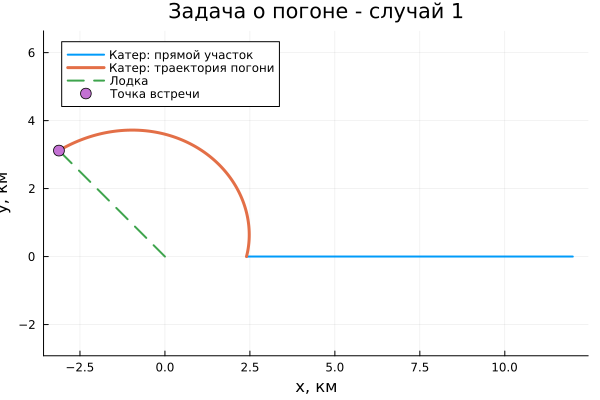
\includegraphics[width=0.76\linewidth,height=\textheight,keepaspectratio]{image/case1.png}

Начальный радиус:

\[
r_0=2.4\text{ км}.
\]

Точка встречи:

\[
\boxed{(-3.1182;\;3.1182)}
\]
\end{frame}

\begin{frame}{Второй случай}
\protect\phantomsection\label{ux432ux442ux43eux440ux43eux439-ux441ux43bux443ux447ux430ux439}
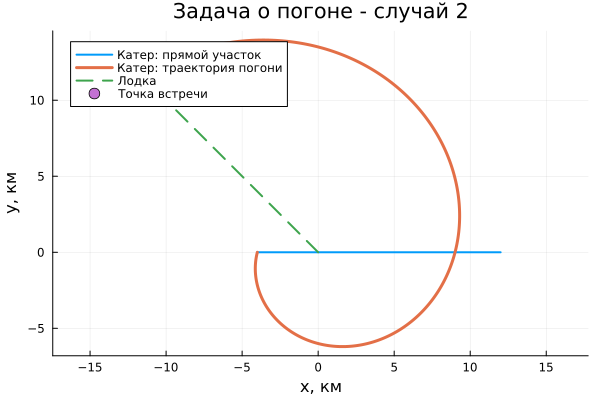
\includegraphics[width=0.76\linewidth,height=\textheight,keepaspectratio]{image/case2.png}

Начальный радиус:

\[
r_0=4\text{ км}.
\]

Точка встречи:

\[
\boxed{(-11.6960;\;11.6960)}
\]
\end{frame}

\begin{frame}{Сравнение результатов}
\protect\phantomsection\label{ux441ux440ux430ux432ux43dux435ux43dux438ux435-ux440ux435ux437ux443ux43bux44cux442ux430ux442ux43eux432}
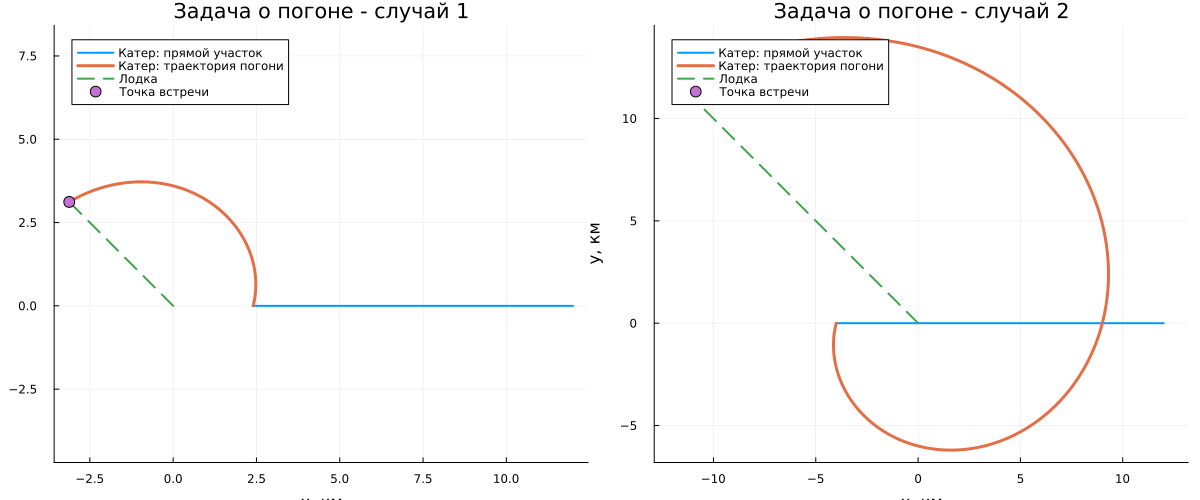
\includegraphics[width=0.9\linewidth,height=\textheight,keepaspectratio]{image/both_cases.png}

В обоих случаях используется одно уравнение движения.

Различие траекторий определяется начальными условиями.
\end{frame}

\begin{frame}{Итог}
\protect\phantomsection\label{ux438ux442ux43eux433}
Для варианта 2:

\[
k=12\text{ км}, \qquad n=4.
\]

Получено уравнение

\[
\frac{dr}{d\theta}=\frac{r}{\sqrt{15}}.
\]

Для двух начальных положений:

\begin{itemize}
\tightlist
\item
  построены траектории катера и лодки;
\item
  определены точки их пересечения;
\item
  получены разные траектории при одном уравнении движения.
\end{itemize}
\end{frame}




\end{document}
